\documentclass{standalone}
\usepackage{tikz}
\usetikzlibrary{patterns, positioning}


\begin{document}
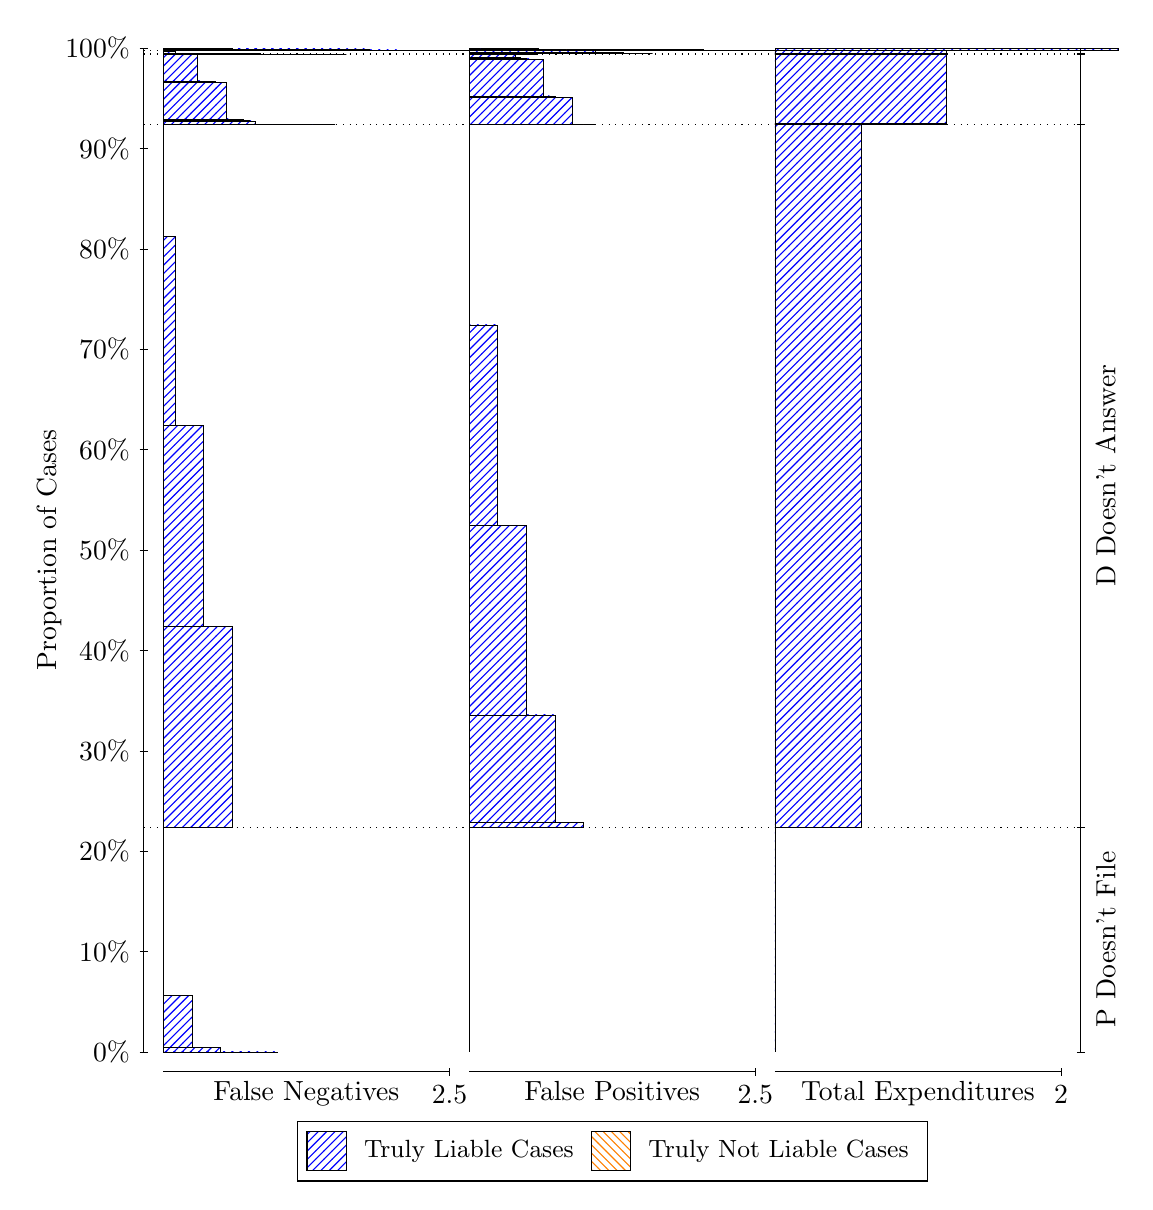
\begin{tikzpicture}
\draw[black, very thin] (1.5,1.75) -- (1.5,14.5);
\node[rotate=90, text=black, anchor=center] at (0.3, 8.125) {Proportion of Cases};
\draw[black, very thin] (1.45,1.75) -- (1.55,1.75);
\node[text=black, anchor=east] at (1.45, 1.75) {0\%};
\draw[black, very thin] (1.45,3.025) -- (1.55,3.025);
\node[text=black, anchor=east] at (1.45, 3.025) {10\%};
\draw[black, very thin] (1.45,4.3) -- (1.55,4.3);
\node[text=black, anchor=east] at (1.45, 4.3) {20\%};
\draw[black, very thin] (1.45,5.575) -- (1.55,5.575);
\node[text=black, anchor=east] at (1.45, 5.575) {30\%};
\draw[black, very thin] (1.45,6.85) -- (1.55,6.85);
\node[text=black, anchor=east] at (1.45, 6.85) {40\%};
\draw[black, very thin] (1.45,8.125) -- (1.55,8.125);
\node[text=black, anchor=east] at (1.45, 8.125) {50\%};
\draw[black, very thin] (1.45,9.4) -- (1.55,9.4);
\node[text=black, anchor=east] at (1.45, 9.4) {60\%};
\draw[black, very thin] (1.45,10.675) -- (1.55,10.675);
\node[text=black, anchor=east] at (1.45, 10.675) {70\%};
\draw[black, very thin] (1.45,11.95) -- (1.55,11.95);
\node[text=black, anchor=east] at (1.45, 11.95) {80\%};
\draw[black, very thin] (1.45,13.225) -- (1.55,13.225);
\node[text=black, anchor=east] at (1.45, 13.225) {90\%};
\draw[black, very thin] (1.45,14.5) -- (1.55,14.5);
\node[text=black, anchor=east] at (1.45, 14.5) {100\%};

\draw[black, very thin] (13.4,1.75) -- (13.4,14.5);
\draw[black, very thin] (13.35,1.75) -- (13.45,1.75);
\node[anchor=west] at (13.35, 1.75) {};
\draw[black, very thin] (13.35,4.6045) -- (13.45,4.6045);
\node[anchor=west] at (13.35, 4.6045) {};
\draw[black, very thin] (13.35,13.534) -- (13.45,13.534);
\node[anchor=west] at (13.35, 13.534) {};
\draw[black, very thin] (13.35,14.42) -- (13.45,14.42);
\node[anchor=west] at (13.35, 14.42) {};
\draw[black, very thin] (13.35,14.431) -- (13.45,14.431);
\node[anchor=west] at (13.35, 14.431) {};
\draw[black, very thin] (13.35,14.471) -- (13.45,14.471);
\node[anchor=west] at (13.35, 14.471) {};
\draw[black, very thin] (13.35,14.5) -- (13.45,14.5);
\node[anchor=west] at (13.35, 14.5) {};

\draw[black, very thin, pattern color=blue, pattern=north east lines] (1.75,1.75) rectangle (3.2033,1.75);
\draw[black, very thin, pattern color=blue, pattern=north east lines] (1.75,1.75) rectangle (2.84,1.7505);
\draw[black, very thin, pattern color=blue, pattern=north east lines] (1.75,1.7505) rectangle (2.4767,1.8121);
\draw[black, very thin, pattern color=blue, pattern=north east lines] (1.75,1.8121) rectangle (2.1133,2.4663);
\draw[black, very thin, pattern color=orange, pattern=north west lines] (1.75,2.4663) rectangle (1.75,2.4663);
\draw[black, very thin, pattern color=blue, pattern=north east lines] (1.75,2.4663) rectangle (1.75,4.6045);
\draw[black, very thin, pattern color=blue, pattern=north east lines] (1.75,4.6045) rectangle (2.622,7.1544);
\draw[black, very thin, pattern color=blue, pattern=north east lines] (1.75,7.1544) rectangle (2.2587,9.7032);
\draw[black, very thin, pattern color=blue, pattern=north east lines] (1.75,9.7032) rectangle (1.8953,12.107);
\draw[black, very thin, pattern color=orange, pattern=north west lines] (1.75,12.107) rectangle (1.75,12.107);
\draw[black, very thin, pattern color=blue, pattern=north east lines] (1.75,12.107) rectangle (1.75,13.534);
\draw[black, very thin, pattern color=blue, pattern=north east lines] (1.75,13.534) rectangle (3.93,13.534);
\draw[black, very thin, pattern color=blue, pattern=north east lines] (1.75,13.534) rectangle (3.7847,13.534);
\draw[black, very thin, pattern color=blue, pattern=north east lines] (1.75,13.534) rectangle (3.6393,13.534);
\draw[black, very thin, pattern color=blue, pattern=north east lines] (1.75,13.534) rectangle (3.5667,13.534);
\draw[black, very thin, pattern color=blue, pattern=north east lines] (1.75,13.534) rectangle (3.494,13.534);
\draw[black, very thin, pattern color=blue, pattern=north east lines] (1.75,13.534) rectangle (3.4213,13.534);
\draw[black, very thin, pattern color=blue, pattern=north east lines] (1.75,13.534) rectangle (3.3487,13.534);
\draw[black, very thin, pattern color=blue, pattern=north east lines] (1.75,13.534) rectangle (3.276,13.534);
\draw[black, very thin, pattern color=blue, pattern=north east lines] (1.75,13.534) rectangle (3.2033,13.534);
\draw[black, very thin, pattern color=blue, pattern=north east lines] (1.75,13.534) rectangle (3.1307,13.534);
\draw[black, very thin, pattern color=blue, pattern=north east lines] (1.75,13.534) rectangle (3.058,13.534);
\draw[black, very thin, pattern color=blue, pattern=north east lines] (1.75,13.534) rectangle (2.9853,13.535);
\draw[black, very thin, pattern color=blue, pattern=north east lines] (1.75,13.535) rectangle (2.9127,13.575);
\draw[black, very thin, pattern color=blue, pattern=north east lines] (1.75,13.575) rectangle (2.84,13.581);
\draw[black, very thin, pattern color=blue, pattern=north east lines] (1.75,13.581) rectangle (2.7673,13.591);
\draw[black, very thin, pattern color=blue, pattern=north east lines] (1.75,13.591) rectangle (2.6947,13.595);
\draw[black, very thin, pattern color=blue, pattern=north east lines] (1.75,13.595) rectangle (2.622,13.6);
\draw[black, very thin, pattern color=blue, pattern=north east lines] (1.75,13.6) rectangle (2.5493,14.062);
\draw[black, very thin, pattern color=blue, pattern=north east lines] (1.75,14.062) rectangle (2.4767,14.07);
\draw[black, very thin, pattern color=blue, pattern=north east lines] (1.75,14.07) rectangle (2.404,14.08);
\draw[black, very thin, pattern color=blue, pattern=north east lines] (1.75,14.08) rectangle (2.3313,14.08);
\draw[black, very thin, pattern color=blue, pattern=north east lines] (1.75,14.08) rectangle (2.2587,14.083);
\draw[black, very thin, pattern color=blue, pattern=north east lines] (1.75,14.083) rectangle (2.186,14.42);
\draw[black, very thin, pattern color=blue, pattern=north east lines] (1.75,14.42) rectangle (2.0407,14.42);
\draw[black, very thin, pattern color=blue, pattern=north east lines] (1.75,14.42) rectangle (1.8953,14.42);
\draw[black, very thin, pattern color=orange, pattern=north west lines] (1.75,14.42) rectangle (1.75,14.42);
\draw[black, very thin, pattern color=blue, pattern=north east lines] (1.75,14.42) rectangle (4.0753,14.42);
\draw[black, very thin, pattern color=blue, pattern=north east lines] (1.75,14.42) rectangle (3.712,14.42);
\draw[black, very thin, pattern color=blue, pattern=north east lines] (1.75,14.42) rectangle (3.3487,14.421);
\draw[black, very thin, pattern color=blue, pattern=north east lines] (1.75,14.421) rectangle (2.9853,14.431);
\draw[black, very thin, pattern color=blue, pattern=north east lines] (1.75,14.431) rectangle (2.622,14.431);
\draw[black, very thin, pattern color=orange, pattern=north west lines] (1.75,14.431) rectangle (1.75,14.431);
\draw[black, very thin, pattern color=blue, pattern=north east lines] (1.75,14.431) rectangle (2.622,14.431);
\draw[black, very thin, pattern color=blue, pattern=north east lines] (1.75,14.431) rectangle (2.2587,14.432);
\draw[black, very thin, pattern color=blue, pattern=north east lines] (1.75,14.432) rectangle (1.8953,14.456);
\draw[black, very thin, pattern color=orange, pattern=north west lines] (1.75,14.456) rectangle (1.75,14.456);
\draw[black, very thin, pattern color=blue, pattern=north east lines] (1.75,14.456) rectangle (1.75,14.471);
\draw[black, very thin, pattern color=blue, pattern=north east lines] (1.75,14.471) rectangle (5.8193,14.471);
\draw[black, very thin, pattern color=blue, pattern=north east lines] (1.75,14.471) rectangle (5.456,14.471);
\draw[black, very thin, pattern color=blue, pattern=north east lines] (1.75,14.471) rectangle (5.0927,14.471);
\draw[black, very thin, pattern color=blue, pattern=north east lines] (1.75,14.471) rectangle (4.7293,14.477);
\draw[black, very thin, pattern color=blue, pattern=north east lines] (1.75,14.477) rectangle (4.366,14.489);
\draw[black, very thin, pattern color=blue, pattern=north east lines] (1.75,14.489) rectangle (4.0027,14.489);
\draw[black, very thin, pattern color=blue, pattern=north east lines] (1.75,14.489) rectangle (3.712,14.489);
\draw[black, very thin, pattern color=blue, pattern=north east lines] (1.75,14.489) rectangle (3.3487,14.489);
\draw[black, very thin, pattern color=blue, pattern=north east lines] (1.75,14.489) rectangle (2.9853,14.489);
\draw[black, very thin, pattern color=blue, pattern=north east lines] (1.75,14.489) rectangle (2.622,14.493);
\draw[black, very thin, pattern color=blue, pattern=north east lines] (1.75,14.493) rectangle (2.2587,14.499);
\draw[black, very thin, pattern color=blue, pattern=north east lines] (1.75,14.499) rectangle (1.8953,14.5);
\draw[black, very thin, pattern color=orange, pattern=north west lines] (1.75,14.5) rectangle (1.75,14.5);
\draw[black, very thin, pattern color=blue, pattern=north east lines] (1.75,14.5) rectangle (1.75,14.5);
\draw[black, very thin, pattern color=orange, pattern=north west lines] (5.6333,1.75) rectangle (5.6333,1.75);
\draw[black, very thin, pattern color=blue, pattern=north east lines] (5.6333,1.75) rectangle (5.6333,4.6045);
\draw[black, very thin, pattern color=orange, pattern=north west lines] (5.6333,4.6045) rectangle (7.0867,4.6045);
\draw[black, very thin, pattern color=blue, pattern=north east lines] (5.6333,4.6045) rectangle (7.0867,4.6689);
\draw[black, very thin, pattern color=blue, pattern=north east lines] (5.6333,4.6689) rectangle (6.7233,6.0314);
\draw[black, very thin, pattern color=blue, pattern=north east lines] (5.6333,6.0314) rectangle (6.36,8.4354);
\draw[black, very thin, pattern color=blue, pattern=north east lines] (5.6333,8.4354) rectangle (5.9967,10.984);
\draw[black, very thin, pattern color=blue, pattern=north east lines] (5.6333,10.984) rectangle (5.6333,13.534);
\draw[black, very thin, pattern color=orange, pattern=north west lines] (5.6333,13.534) rectangle (7.232,13.534);
\draw[black, very thin, pattern color=blue, pattern=north east lines] (5.6333,13.534) rectangle (7.232,13.534);
\draw[black, very thin, pattern color=orange, pattern=north west lines] (5.6333,13.534) rectangle (7.0867,13.534);
\draw[black, very thin, pattern color=blue, pattern=north east lines] (5.6333,13.534) rectangle (7.0867,13.534);
\draw[black, very thin, pattern color=orange, pattern=north west lines] (5.6333,13.534) rectangle (6.9413,13.534);
\draw[black, very thin, pattern color=blue, pattern=north east lines] (5.6333,13.534) rectangle (6.9413,13.871);
\draw[black, very thin, pattern color=blue, pattern=north east lines] (5.6333,13.871) rectangle (6.8687,13.873);
\draw[black, very thin, pattern color=orange, pattern=north west lines] (5.6333,13.873) rectangle (6.796,13.873);
\draw[black, very thin, pattern color=blue, pattern=north east lines] (5.6333,13.873) rectangle (6.796,13.874);
\draw[black, very thin, pattern color=blue, pattern=north east lines] (5.6333,13.874) rectangle (6.7233,13.883);
\draw[black, very thin, pattern color=orange, pattern=north west lines] (5.6333,13.883) rectangle (6.6507,13.883);
\draw[black, very thin, pattern color=blue, pattern=north east lines] (5.6333,13.883) rectangle (6.6507,13.892);
\draw[black, very thin, pattern color=blue, pattern=north east lines] (5.6333,13.892) rectangle (6.578,14.353);
\draw[black, very thin, pattern color=blue, pattern=north east lines] (5.6333,14.353) rectangle (6.5053,14.358);
\draw[black, very thin, pattern color=blue, pattern=north east lines] (5.6333,14.358) rectangle (6.4327,14.363);
\draw[black, very thin, pattern color=blue, pattern=north east lines] (5.6333,14.363) rectangle (6.36,14.372);
\draw[black, very thin, pattern color=blue, pattern=north east lines] (5.6333,14.372) rectangle (6.2873,14.379);
\draw[black, very thin, pattern color=blue, pattern=north east lines] (5.6333,14.379) rectangle (6.2147,14.419);
\draw[black, very thin, pattern color=blue, pattern=north east lines] (5.6333,14.419) rectangle (6.142,14.419);
\draw[black, very thin, pattern color=blue, pattern=north east lines] (5.6333,14.419) rectangle (6.0693,14.419);
\draw[black, very thin, pattern color=blue, pattern=north east lines] (5.6333,14.419) rectangle (5.9967,14.419);
\draw[black, very thin, pattern color=blue, pattern=north east lines] (5.6333,14.419) rectangle (5.924,14.42);
\draw[black, very thin, pattern color=blue, pattern=north east lines] (5.6333,14.42) rectangle (5.8513,14.42);
\draw[black, very thin, pattern color=blue, pattern=north east lines] (5.6333,14.42) rectangle (5.7787,14.42);
\draw[black, very thin, pattern color=blue, pattern=north east lines] (5.6333,14.42) rectangle (5.706,14.42);
\draw[black, very thin, pattern color=blue, pattern=north east lines] (5.6333,14.42) rectangle (5.6333,14.42);
\draw[black, very thin, pattern color=orange, pattern=north west lines] (5.6333,14.42) rectangle (6.5053,14.42);
\draw[black, very thin, pattern color=blue, pattern=north east lines] (5.6333,14.42) rectangle (6.5053,14.42);
\draw[black, very thin, pattern color=blue, pattern=north east lines] (5.6333,14.42) rectangle (6.142,14.429);
\draw[black, very thin, pattern color=blue, pattern=north east lines] (5.6333,14.429) rectangle (5.7787,14.431);
\draw[black, very thin, pattern color=blue, pattern=north east lines] (5.6333,14.431) rectangle (5.6333,14.431);
\draw[black, very thin, pattern color=orange, pattern=north west lines] (5.6333,14.431) rectangle (7.9587,14.431);
\draw[black, very thin, pattern color=blue, pattern=north east lines] (5.6333,14.431) rectangle (7.9587,14.431);
\draw[black, very thin, pattern color=blue, pattern=north east lines] (5.6333,14.431) rectangle (7.5953,14.446);
\draw[black, very thin, pattern color=blue, pattern=north east lines] (5.6333,14.446) rectangle (7.232,14.47);
\draw[black, very thin, pattern color=blue, pattern=north east lines] (5.6333,14.47) rectangle (6.8687,14.471);
\draw[black, very thin, pattern color=blue, pattern=north east lines] (5.6333,14.471) rectangle (6.5053,14.471);
\draw[black, very thin, pattern color=orange, pattern=north west lines] (5.6333,14.471) rectangle (9.7027,14.471);
\draw[black, very thin, pattern color=blue, pattern=north east lines] (5.6333,14.471) rectangle (9.7027,14.471);
\draw[black, very thin, pattern color=orange, pattern=north west lines] (5.6333,14.471) rectangle (9.3393,14.471);
\draw[black, very thin, pattern color=blue, pattern=north east lines] (5.6333,14.471) rectangle (9.3393,14.471);
\draw[black, very thin, pattern color=orange, pattern=north west lines] (5.6333,14.471) rectangle (8.976,14.471);
\draw[black, very thin, pattern color=blue, pattern=north east lines] (5.6333,14.471) rectangle (8.976,14.472);
\draw[black, very thin, pattern color=orange, pattern=north west lines] (5.6333,14.472) rectangle (8.6127,14.472);
\draw[black, very thin, pattern color=blue, pattern=north east lines] (5.6333,14.472) rectangle (8.6127,14.478);
\draw[black, very thin, pattern color=blue, pattern=north east lines] (5.6333,14.478) rectangle (8.2493,14.481);
\draw[black, very thin, pattern color=blue, pattern=north east lines] (5.6333,14.481) rectangle (7.886,14.482);
\draw[black, very thin, pattern color=blue, pattern=north east lines] (5.6333,14.482) rectangle (7.5227,14.482);
\draw[black, very thin, pattern color=blue, pattern=north east lines] (5.6333,14.482) rectangle (7.1593,14.482);
\draw[black, very thin, pattern color=orange, pattern=north west lines] (5.6333,14.482) rectangle (6.8687,14.482);
\draw[black, very thin, pattern color=blue, pattern=north east lines] (5.6333,14.482) rectangle (6.8687,14.482);
\draw[black, very thin, pattern color=orange, pattern=north west lines] (5.6333,14.482) rectangle (6.5053,14.482);
\draw[black, very thin, pattern color=blue, pattern=north east lines] (5.6333,14.482) rectangle (6.5053,14.494);
\draw[black, very thin, pattern color=blue, pattern=north east lines] (5.6333,14.494) rectangle (6.142,14.5);
\draw[black, very thin, pattern color=blue, pattern=north east lines] (5.6333,14.5) rectangle (5.7787,14.5);
\draw[black, very thin, pattern color=blue, pattern=north east lines] (5.6333,14.5) rectangle (5.6333,14.5);
\draw[black, very thin, pattern color=orange, pattern=north west lines] (9.5167,1.75) rectangle (9.5167,1.75);
\draw[black, very thin, pattern color=blue, pattern=north east lines] (9.5167,1.75) rectangle (9.5167,4.6045);
\draw[black, very thin, pattern color=orange, pattern=north west lines] (9.5167,4.6045) rectangle (10.607,4.6045);
\draw[black, very thin, pattern color=blue, pattern=north east lines] (9.5167,4.6045) rectangle (10.607,13.534);
\draw[black, very thin, pattern color=orange, pattern=north west lines] (9.5167,13.534) rectangle (11.697,13.534);
\draw[black, very thin, pattern color=blue, pattern=north east lines] (9.5167,13.534) rectangle (11.697,13.542);
\draw[black, very thin, pattern color=orange, pattern=north west lines] (9.5167,13.542) rectangle (11.697,13.542);
\draw[black, very thin, pattern color=blue, pattern=north east lines] (9.5167,13.542) rectangle (11.697,14.42);
\draw[black, very thin, pattern color=orange, pattern=north west lines] (9.5167,14.42) rectangle (11.697,14.42);
\draw[black, very thin, pattern color=blue, pattern=north east lines] (9.5167,14.42) rectangle (11.697,14.431);
\draw[black, very thin, pattern color=orange, pattern=north west lines] (9.5167,14.431) rectangle (11.697,14.431);
\draw[black, very thin, pattern color=blue, pattern=north east lines] (9.5167,14.431) rectangle (11.697,14.471);
\draw[black, very thin, pattern color=orange, pattern=north west lines] (9.5167,14.471) rectangle (13.877,14.471);
\draw[black, very thin, pattern color=blue, pattern=north east lines] (9.5167,14.471) rectangle (13.877,14.5);
\draw[black, dotted] (1.5,4.6045) -- (13.4,4.6045);
\draw[black, dotted] (1.5,13.534) -- (13.4,13.534);
\draw[black, dotted] (1.5,14.42) -- (13.4,14.42);
\draw[black, dotted] (1.5,14.431) -- (13.4,14.431);
\draw[black, dotted] (1.5,14.471) -- (13.4,14.471);
\draw[black, very thin] (1.75,1.5) -- (5.3833,1.5);
\node[text=black, anchor=north] at (3.5667, 1.5) {False Negatives};
\draw[black, very thin] (5.3833,1.45) -- (5.3833,1.55);
\node[text=black, anchor=north] at (5.3833, 1.45) {2.5};

\draw[black, very thin] (5.6333,1.5) -- (9.2667,1.5);
\node[text=black, anchor=north] at (7.45, 1.5) {False Positives};
\draw[black, very thin] (9.2667,1.45) -- (9.2667,1.55);
\node[text=black, anchor=north] at (9.2667, 1.45) {2.5};

\draw[black, very thin] (9.5167,1.5) -- (13.15,1.5);
\node[text=black, anchor=north] at (11.333, 1.5) {Total Expenditures};
\draw[black, very thin] (13.15,1.45) -- (13.15,1.55);
\node[text=black, anchor=north] at (13.15, 1.45) {2};

\node[text=black, centered, rotate=90] at (13.72, 3.1773) {P Doesn't File};
\node[text=black, centered, rotate=90] at (13.72, 9.0693) {D Doesn't Answer};





\draw (7.449999999999999,1.5) node[draw=none] (baseCoordinate) {};
\begin{scope}[align=center]
        \matrix[scale=0.5, draw=black, below=0.5cm of baseCoordinate, nodes={draw}, column sep=0.1cm]{
            \node[rectangle, draw, minimum width=0.5cm, minimum height=0.5cm, pattern color=blue, pattern=north east lines] {}; &
            \node[draw=none, font=\small, text=black] (B) {Truly Liable Cases}; &
            \node[rectangle, draw, minimum width=0.5cm, minimum height=0.5cm, pattern color=orange, pattern=north west lines] {}; &
            \node[draw=none, font=\small, text=black] (B) {Truly Not Liable Cases}; \\
            };
\end{scope}

\end{tikzpicture}
\end{document}